\documentclass[final,5p,times,twocolumn,authoryear]{elsarticle}

\usepackage{amsmath,amssymb}
\usepackage{booktabs}
\usepackage{graphicx}
\usepackage[hidelinks]{hyperref}

\newcommand{\ddx}[2]{\frac{\partial #1}{\partial #2}}
\newcommand{\dd}{\,\mathrm{d}}
\newcommand{\I}{\mathrm{i}}
\newcommand{\gbar}{\bar{g}}

\journal{Journal of Mathematical Psychology}

\begin{document}

\begin{frontmatter}

\title{The first-passage time density for the diffusion model with variable drift and variable starting point}

\author{Kiant\'e Fernandez\corref{cor1}}
\ead{kiante@ucla.edu}
\address{Department of Psychology, University of California, Los Angeles, 1285 Franz Hall, Los Angeles, CA 90095, United States}
\cortext[cor1]{Corresponding author.}

\begin{abstract}
The Ratcliff diffusion model is fitted with across-trial variability in drift rate, starting point, and non-decision time. The drift integral of the first-passage time density has been evaluated in closed form at fixed starting point, and the starting-point and non-decision-time integrals at fixed drift, but the drift and starting-point integrals have not been evaluated together. In particular, existing software implementations integrate at least one of these two numerically. We show that in the small-time series representation the starting-point integral of the drift-integrated density is an integral of a linear function against a normal density, and we give the density with normally distributed drift and uniformly distributed starting point in closed form together with a large-time counterpart in terms of the complex error function. The six-parameter density then requires no numerical integration at all, and the seven-parameter likelihood a single one-dimensional quadrature. The derivatives of the density with respect to all of its parameters follow in closed form, and the likelihood gradient reuses that one quadrature. The result is verified symbolically and against three reference implementations, and is machine-checked in Lean.
\end{abstract}

\begin{keyword}
Diffusion model \sep Response time modeling \sep First-passage time \sep Starting point variability
\end{keyword}

\end{frontmatter}


\section{Background}

The diffusion model for response times \citep{Ratcliff1978} describes a two-choice decision as a Wiener process with drift $v$ and unit diffusion coefficient\footnote{For diffusion coefficient $\sigma^2 \neq 1$ all results below hold after the substitution $(v, \eta^2, a) \to (v/\sigma, \eta^2/\sigma^2, a/\sigma)$ \citep{Blurton2017}.} evolving between two absorbing barriers at $0$ and $a > 0$ from a starting point $aw$, $0 < w < 1$. The first-passage times at the two barriers are the predicted response times for the two alternatives. To account for the fast and slow errors observed in most speeded response experiments, the model is applied with across-trial variability in three of its quantities \citep{Ratcliff1978, RatcliffRouder1998, RatcliffTuerlinckx2002, RatcliffMcKoon2008}: the drift rate is normally distributed, $v \sim N(\nu, \eta^2)$; the starting point is uniformly distributed, $w \sim U(w_1, w_2)$, with Ratcliff's $s_z = a(w_2 - w_1)$; and the non-decision time is uniformly distributed over a window of width $s_t$. The predicted density of a response time is then a triple integral of the constant-parameter first-passage time density over these three distributions. The decision-time density derived below has five parameters, $\nu$, $\eta$, $a$, and the endpoints $w_1, w_2$ of the starting-point range, which replace Ratcliff's $w = (w_1 + w_2)/2$ and $s_z$; a fixed non-decision time $t_0$ shifts its argument and gives the six-parameter model, and the width $s_t$ the seven-parameter model.

The drift integral has been closed at fixed starting point, and the starting-point and non-decision-time integrals at fixed drift, but the drift and starting-point integrals have not been closed together. The first-passage time density with normally distributed drift is given by \citet{HorrocksThompson2004} and, for the lower barrier, reads \citep[Eq.~1]{Blurton2017}
\begin{align}
g\left(t \mid \nu, \eta^2, a, w\right)
 &= \frac{1}{\sqrt{2\pi t^3 S}}
   \exp\!\left[\frac{-\nu^2 t - 2\nu a w + \eta^2 (a w)^2}{2S}\right] \notag\\
 &\quad\times \sum_{j=0}^{\infty} (-1)^j\, r_j \exp\!\left(-\frac{r_j^2}{2t}\right),
\label{eq:geta}
\end{align}
where $S := 1 + \eta^2 t$, $r_j = ja + aw$ for even $j$ and $r_j = ja + a(1-w)$ for odd $j$. \citet{Blurton2017} derived the corresponding cumulative distribution function. Both results are stated in the small-time series representation of the first-passage time density \citep{Hall1997, VanZandt2000, NavarroFuss2009, Blurton2012, Gondan2014}, that is, as a series whose $j$th term carries the standard normal density evaluated at $r_j/\sqrt t$, the factor $\exp(-r_j^2/(2t))$ in~\eqref{eq:geta}.

The remaining two integrals close at fixed drift. \citet[pp.~706--708]{Tuerlinckx2004} worked in the large-time representation of \citet{Ratcliff1978}, in which the starting point enters through $\sin(k\pi w)$, integrated the starting point and the non-decision time analytically at fixed drift, and found that the drift integral has to be approximated by quadrature (software like DMAT \citep{VandekerckhoveTuerlinckx2008} follows this route). Every implementation of the density we are aware of starts instead from the drift-integrated density~\eqref{eq:geta} and integrates the starting point numerically: fast-dm and rtdists \citep{VossVoss2007, Singmann2022}, HDDM \citep{Wiecki2013}, WienR \citep{HartmannKlauer2021, WienR}, and the Stan implementation of \citet{Henrich2024}. The recent monograph of \citet[Section~4.5]{SmithRatcliff2025} likewise carries out only the drift integral analytically. \citet{Blurton2017} noted that adding starting-point and non-decision-time variability to their result ``requires numerical evaluation of two integrals'' (p.~11).

In this note we show that the starting-point integral of the density~\eqref{eq:geta} has a closed form and that what the integral turns into depends on the series representation. In the large-time series, once the drift has been integrated, the starting point appears in a Gaussian factor with a \emph{positive} coefficient of $w^2$, and the integral against $\sin(k\pi w)$ is an imaginary error function of complex argument, which is rewritten through the Faddeeva function (Section~\ref{sec:large}). In the small-time series the factor $\exp(-r_j^2/(2t))$ contributes a negative coefficient of $w^2$ that always dominates the positive one produced by the drift integral, so the integrand is a linear function times a decaying Gaussian, and the integral is a Gaussian moment with a closed form. Section~\ref{sec:result} gives the result and its derivation, Section~\ref{sec:large} the large-time counterpart that is needed for numerical stability at large $t$, Section~\ref{sec:conv} the truncation rule, and Section~\ref{sec:verify} the numerical verification and a comparison with existing software.

\section{The density with variable drift and variable starting point}
\label{sec:result}

Let the starting point be uniformly distributed on $[w_1, w_2]$ with $0 < w_1 \le w_2 < 1$. Equation~\eqref{eq:result} is defined at $w_1 = 0$ as well, where the density has an integrable singularity of order $t^{-1/2}$ as $t \to 0$; existing implementations exclude that point, rejecting the input or returning zero. The lower-barrier first-passage time defective density of the resulting process is
\begin{equation}
\gbar\left(t \mid \nu, \eta^2, a, w_1, w_2\right) := \frac{1}{w_2 - w_1}\int_{w_1}^{w_2} g\left(t \mid \nu, \eta^2, a, w\right) \dd w .
\label{eq:def}
\end{equation}
The series in~\eqref{eq:geta} converges absolutely and uniformly in $w$ (\ref{app:bound}), so summation and integration may be exchanged and it suffices to integrate one term.

\subsection{The $j$-th term is a Gaussian moment}

Write $r_j = p_j + q_j w$ with $p_j = ja$, $q_j = a$ for even $j$, and $p_j = (j+1)a$, $q_j = -a$ for odd $j$. Collecting the exponentials of the $j$-th term of~\eqref{eq:geta}, that is, of $\exp[(-\nu^2 t - 2\nu a w + \eta^2 a^2 w^2)/2S]\, r_j \exp(-r_j^2/(2t))$, gives a quadratic exponent in $w$,
\begin{equation}
(p_j + q_j w)\exp\!\left(-\tfrac{1}{2} A w^2 + B_j w + C_j\right),
\label{eq:term}
\end{equation}
with
\begin{align}
A &= \frac{a^2}{tS}, \qquad
B_j = -\frac{\nu a}{S} - \frac{p_j q_j}{t}, \qquad
C_j = -\frac{\nu^2 t}{2S} - \frac{p_j^2}{2t}.
\label{eq:coef}
\end{align}
The coefficient of $w^2$ deserves attention. The drift integral contributes $+\eta^2 a^2/(2S)$, a growing Gaussian in $w$, whereas the factor $\exp(-r_j^2/(2t))$ contributes $-a^2/(2t)$, and
\begin{equation}
\frac{a^2}{2t} - \frac{\eta^2 a^2}{2S} = \frac{a^2 (S - \eta^2 t)}{2tS} = \frac{a^2}{2tS} > 0
\label{eq:key}
\end{equation}
for every $t > 0$ and every $\eta$, and the coefficient does not depend on $j$. The combined exponent is therefore a decaying Gaussian with $A > 0$. Therefore, in the small-time representation, the starting-point integrand is a linear function times a proper Gaussian, and such integrals have closed forms in terms of $\exp$ and $\Phi$.

\subsection{The density in closed form}

For $A > 0$ and $m := B/A$,
\begin{align}
&\int_{w_1}^{w_2} (p + q w)\, \exp(-\tfrac12 A w^2 + B w + C) \dd w \notag\\
 &\quad = (p + q m)\sqrt{\frac{2\pi}{A}}\, \exp(C + B^2/(2A)) \notag\\
 &\qquad\quad\times \left[\Phi\!\big(\sqrt{A}(w_2 - m)\big) - \Phi\!\big(\sqrt{A}(w_1 - m)\big)\right] \notag\\
 &\qquad - \frac{q}{A}\left[\exp(C + B w_2 - \tfrac12 A w_2^2) \right. \notag\\
 &\qquad\qquad\quad \left. - \exp(C + B w_1 - \tfrac12 A w_1^2)\right],
\label{eq:lemma}
\end{align}
where $\Phi$ denotes the standard normal distribution function (\ref{app:lemma}). Applying~\eqref{eq:lemma} term by term with the coefficients~\eqref{eq:coef} gives the lower-barrier first-passage time density with normally distributed drift and uniformly distributed starting point,
\begin{align}
\gbar\left(t \mid \nu, \eta^2, a, w_1, w_2\right)
 &= \frac{1}{(w_2 - w_1)\sqrt{2\pi t^3 S}}\sum_{j=0}^{\infty} (-1)^j I_j , \label{eq:result}\\
I_j &= \int_{w_1}^{w_2} (p_j + q_j w) \notag\\
    &\qquad\times \exp(-\tfrac12 A w^2 + B_j w + C_j)\, \dd w , \notag
\end{align}
with $I_j$ given in closed form by~\eqref{eq:lemma}. The density at the upper barrier is $\gbar(t \mid -\nu, \eta^2, a, 1 - w_2, 1 - w_1)$. Like~\eqref{eq:geta} it is a defective density, integrating over $t$ to the probability of a lower-barrier response rather than to one. For $w_2 - w_1 \to 0$ the result reduces to~\eqref{eq:geta}, and for $\eta = 0$ to the starting-point integral of the constant-drift density, so it can be used in a fitting routine regardless of whether either form of variability is present in the data. We note that like~\eqref{eq:geta}, the density is still an infinite series. Nonetheless what is in closed form is each of its terms, so that no numerical integration over the starting point remains.

For large $j$ the center $m = B_j/A$ of the Gaussian in~\eqref{eq:lemma} lies far outside $[w_1, w_2]$, so $\exp(C + B^2/(2A))$ is very large and the difference of $\Phi$ values very small. The product has to be formed in one step: in log space, as $\exp\{C + B^2/(2A) + \log[\Phi(x_2) - \Phi(x_1)]\}$ with $x_i = \sqrt A(w_i - m)$ and the difference taken on the tail where both $x_i$ lie, or through the scaled complementary error function $\exp(x^2)\operatorname{erfc}(x)$. The two implementations of Section~\ref{sec:verify} use one each and agree to eleven relative digits.

\section{Large-time representation}
\label{sec:large}

Like every small-time series, \eqref{eq:result} loses precision through cancellation when $t/a^2$ is large; in double precision the loss becomes visible for $t/a^2 \gtrsim 2$. A large-time counterpart is obtained from the large-time series of \citet{Ratcliff1978}. Integrating $\exp(-vaw - v^2 t/2)$ against the $N(\nu, \eta^2)$ drift density produces exactly the prefactor of~\eqref{eq:geta} \citep[Eqs.~4.54--4.58]{SmithRatcliff2025}, so the large-time density with normally distributed drift is \citep[see also][Eq.~7]{FosterSingmann2021}
\begin{align}
g\left(t \mid \nu, \eta^2, a, w\right)
 &= \frac{\pi}{a^2\sqrt{S}}\exp\!\left[\frac{-\nu^2 t - 2\nu a w + \eta^2 (a w)^2}{2S}\right] \notag\\
 &\quad\times \sum_{k=1}^{\infty} k\, \exp(-k^2\pi^2 t/(2a^2))\sin(k\pi w) .
\label{eq:large}
\end{align}
\begin{sloppypar}
Here no term carries a factor $\exp(-r_j^2/(2t))$ to compensate the growing Gaussian, and the starting-point integral of the $k$-th term is $\int_{w_1}^{w_2} \exp(\kappa w^2 + \lambda w)\sin(k\pi w)\dd w$ with $\kappa = \eta^2 a^2/(2S) > 0$ and $\lambda = -\nu a/S$. Written as the imaginary part of $\int \exp(\kappa w^2 + \mu_k w)\dd w$ with $\mu_k = \lambda + \I k\pi$, the antiderivative is an imaginary error function of complex argument, whose direct evaluation overflows in double precision and loses digits to cancellation. It is, however, bounded when expressed through the Faddeeva function $W(z) = \exp(-z^2)\operatorname{erfc}(-\I z)$ \citep[Eq.~7.1.3]{AbramowitzStegun1964}, written $W$ here rather than the usual $w$ to keep it apart from the starting point:
\end{sloppypar}
{\small
\begin{equation}
\int_{w_1}^{w_2} \exp(\kappa w^2 + \mu_k w)\dd w
 = \frac{-\I\sqrt{\pi}}{2\sqrt{\kappa}}
   \Big[\exp(\kappa w^2 + \mu_k w)\, W\!\big(z_k(w)\big)\Big]_{w_1}^{w_2},
\label{eq:faddeeva}
\end{equation}}%
with $z_k(w) = \sqrt{\kappa}\, w + \mu_k/(2\sqrt{\kappa})$.
Since $\operatorname{Im} z_k = k\pi/(2\sqrt{\kappa}) > 0$, $z_k$ lies in the upper half plane, where $|W(z)| \le 1$ (\ref{app:bound}), and the product with $\exp(\kappa w^2 + \mu_k w)$ is of the size of the integrand. For $\eta = 0$, where $\kappa = 0$, the right-hand side of~\eqref{eq:faddeeva} is replaced by its $\kappa \to 0$ limit, $(\exp(\mu_k w_2) - \exp(\mu_k w_1))/\mu_k$, which follows from $W(z) \sim \I/(\sqrt\pi z)$ for large $|z|$. The large-time density with uniformly distributed starting point is then
\begin{align}
\gbar\left(t \mid \nu, \eta^2, a, w_1, w_2\right)
 &= \frac{\pi\, \exp(-\nu^2 t/(2S))}{a^2\sqrt{S}\,(w_2 - w_1)} \notag\\
 &\qquad\times \sum_{k=1}^{\infty} k\, \exp(-k^2\pi^2 t/(2a^2)) \notag\\
 &\qquad\times \operatorname{Im}\!\int_{w_1}^{w_2} \exp(\kappa w^2 + \mu_k w)\dd w .
\label{eq:result_large}
\end{align}
Fast and accurate algorithms for $W(z)$ are standard \citep{ZaghloulAli2011} and available in scientific libraries.  Equation~\eqref{eq:faddeeva} must be evaluated through $W$. Written with the imaginary error function, it loses about $\pi^2 k^2/(4\kappa)$ in the exponent to cancellation. Our implementation switches from the small- to the large-time form at $t/a^2 = 1$. The choice is not critical: the two forms agree to thirteen relative digits for $0.1 \le t/a^2 \le 1$ and to eleven at $t/a^2 = 2$.

\section{Convergence}
\label{sec:conv}

\begin{sloppypar}
Both series are infinite and are truncated after $J$ terms for~\eqref{eq:result} and $K$ terms for~\eqref{eq:result_large}. The $j$-th term of~\eqref{eq:result} is at most $c\,(j+1)a\exp(-j^2 a^2/(2t))$ in absolute value, and the $k$-th term of~\eqref{eq:result_large} is at most $c'\,k\exp(-k^2\pi^2 t/(2a^2))$, where $c$ and $c'$ do not depend on the index (\ref{app:bound}). Because the small-time series is used only for $t \le a^2$ and the large-time series only for $t \ge a^2$, from $J = 2$ on each bound is at most a tenth of the one before it. The truncation error is therefore at most a small multiple of the first omitted term, with constants given in \ref{app:bound}. The rule below makes the exponential factor of the first omitted term smaller than a tolerance $\varepsilon$ and adds one term to cover the remaining factors, like the criteria of \citet{NavarroFuss2009} and \citet{Gondan2014}. This bounds the absolute error. The relative error can be larger where the density is small, and it is checked numerically in Section~\ref{sec:verify}. The numbers of terms are:
\end{sloppypar}
\begin{equation}
J = \left\lceil \frac{\sqrt{2 t \log(1/\varepsilon)}}{a} \right\rceil + 1,
\qquad
K = \left\lceil a\sqrt{\frac{2\log(1/\varepsilon)}{\pi^2 t}} \right\rceil + 1 .
\label{eq:JK}
\end{equation}

We take $J \ge 2$ always. With $\varepsilon = 10^{-12}$ the small-time series needs $J \le 9$ terms for $t/a^2 \le 1$, and the large-time series needs $K \le 4$ terms for $t/a^2 \ge 1$. Lowering $\varepsilon$ to $10^{-40}$ changes the results on the 400 parameter sets of Section~\ref{sec:verify} only at the level of double-precision rounding. Since $J$ and $K$ depend on $a$ and $t$ only through $t/a^2$, the rule is invariant under Brownian rescaling and controls the error relative to the scale of the density, not as an absolute tolerance.

\section{Verification and efficiency}
\label{sec:verify}

\subsection{Verification}

We checked the result in four independent ways. (i)~Every algebraic step, in particular the antiderivative~\eqref{eq:lemma}, the inequality~\eqref{eq:key}, the coefficient table~\eqref{eq:coef}, the drift integral leading to~\eqref{eq:geta}, and all derivative formulas of \ref{app:grad}, is verified as an exact symbolic identity in a computer algebra system, that is, as $\mathrm{simplify}(\dd F/\dd x - f) = 0$ rather than by numerical agreement. (ii)~In arbitrary-precision arithmetic with at least 100 digits, and with far more series terms than the rule of Section~\ref{sec:conv} requires, \eqref{eq:result} and~\eqref{eq:result_large} agree with quadrature over $w$ of~\eqref{eq:geta} to at least twenty relative digits, at six and four parameter sets respectively. The two double-precision implementations are then compared with the same quadrature, carried to 50 digits and never using the closed form, on 1000 parameter sets. The sets reach starting points within a millionth of either barrier, starting-point ranges of one ten-thousandth, $\eta = 0$, drift rates of $\pm 10$, $t/a^2$ from $0.01$ to $5$, and densities down to the limit of double precision. On most sets both implementations match the reference to the limit of double precision, about fifteen digits, and on the worst set to ten digits. The five derivatives match to at least nine digits. On 14 further sets the true density is smaller than the smallest positive number double precision can hold. Both implementations return zero there, which is the correct double-precision answer, so these sets contribute no digit count. (iii)~On the 400 parameter sets of Table~\ref{tab:grid}, which span twenty orders of magnitude in density, the switched representation agrees with WienR \citep{HartmannKlauer2021} to nine relative digits, and its five partial derivatives agree with WienR's derivative functions to seven. With $t_0$ and $s_t$ added, \eqref{eq:seven} agrees with WienR to ten relative digits for $w_1 \ge 0.1$ (fewer for smaller $w_1$, Table~\ref{tab:w1}), except at the smallest densities, where the two agree to four digits and adaptive quadrature of~\eqref{eq:seven} shows the difference to be WienR's integration error. The parameter values of published fits \citep{tran2021systematic} and a sweep of $w_2 - w_1$ down to zero give the same agreement and no negative density (\ref{app:grids}). (iv)~The derivation of~\eqref{eq:result}, including the antiderivative, the coefficient table, the exchange of summation and integration, and the Faddeeva integral~\eqref{eq:faddeeva}, is formalized and machine-checked in Lean with Mathlib \citep{deMouraUllrich2021, mathlib2020}; the development contains no unproved statement and relies on no axioms beyond Lean's standard ones. The scope is as follows. The representation~\eqref{eq:geta} is a definition there, as it is taken from the literature here; the large-time series~\eqref{eq:large} itself is not formalized, only the identity~\eqref{eq:faddeeva}; the normal distribution function, the complex error function, and $W(z)$ are defined within the development.

\begin{table}[t]
\centering
\caption{The 400 parameter sets of Section~\ref{sec:verify}, drawn with a fixed seed. $t$ is uniform on its interval and every other parameter uniform over its listed values. The seven-parameter sets add $t_0$ and $s_t$ and shift $t$ by $t_0$.}
\label{tab:grid}
\begin{tabular}{ll}
\toprule
Parameter & Values \\
\midrule
$a$ & $0.6$, $1$, $1.5$, $2.5$ \\
$\nu$ & $-3$, $-1$, $-0.2$, $0$, $0.5$, $1.5$, $4$ \\
$\eta$ & $0.5$, $1$, $2$ \\
$(w_1 + w_2)/2$ & $0.3$, $0.5$, $0.7$ \\
$w_2 - w_1$ & $0.05$, $0.2$, $0.4$ \\
$t$ & $[0.05, 3]$ \\
\midrule
$t_0$ & $0.3$ \\
$s_t$ & $0.1$, $0.25$ \\
\bottomrule
\end{tabular}
\end{table}


\subsection{Efficiency}

Table~\ref{tab:timing} compares the cost of~\eqref{eq:result}, in a compiled implementation of the formulas, with three packages in common use: WienR, which evaluates the drift-integrated series by adaptive quadrature over $w$; rtdists, whose (via fast-dm) diffusion code integrates over $w$ and the non-decision window numerically; and the HDDM likelihood \citep{Wiecki2013, hddmwfpt}, which does the same with the Navarro--Fuss series. All timings are single-threaded on one machine,\footnote{Apple M1 Pro; R 4.5.3 with WienR 0.3-15 and rtdists 0.12-0; Python 3.11 with NumPy 1.26.4, SciPy 1.13.1, Cython 3.1.4, and hddm-wfpt 0.1.4.} for 10\,000 response times at one parameter set, which is the situation in a likelihood evaluation.

The difference columns need a reference scale. \citet{Blurton2017} recommend a truncation tolerance of $1.5\times10^{-8}$, the square root of double-precision machine epsilon; \citet{Gondan2014} illustrate their term counts at three decimals; and \citet[Table~1]{Tuerlinckx2004} found his quadrature-based algorithm and the classical one to differ at the fourth to seventh decimal. Among current packages, rtdists (fast-dm) defaults to roughly three accurate decimals, the HDDM likelihood to four for its series and eight for its integrations over the starting point and the non-decision window, the Stan implementation of \citet{Henrich2024} to six for the density and four for its derivatives, and WienR to nine at its default call. Taken together, the truncation tolerance of the closed form, $10^{-12}$, is at or below the default setting of each of these packages; Table~\ref{tab:timing} reports the measured differences for the three that we timed.

\begin{table}[t]
\centering
\caption{Cost and accuracy of the closed form and three packages. Cost is microseconds per evaluation on one thread, over 10\,000 response times drawn uniformly between 0.1 and 3~s, at $a = 1.2$, $\nu = \eta = 1$, $w_1 = 0.4$, and $w_2 = 0.6$. Difference is the largest relative difference from the closed form over the 400 parameter sets of Table~\ref{tab:grid}, counting densities above $0.001$. Each package runs at the settings used for fitting. WienR runs at precision $10^{-12}$, rtdists at precision 3, and HDDM at series precision $10^{-4}$ and Simpson precision $10^{-8}$ with recursion depth 10.}
\label{tab:timing}
\footnotesize
\begin{tabular}{lcc}
\toprule
 & Difference & $\mu$s \\
\midrule
Closed form   & --                 & 0.34 \\
WienR, $10^{-12}$ & $3.8\times10^{-13}$ & 2.2  \\
rtdists       & $4.6\times10^{-3}$ & 0.43 \\
HDDM          & $3.9\times10^{-6}$ & 0.57 \\
\midrule
Closed form $+$ 5 gradients$^{\dagger}$ & --      & 2.3  \\
WienR, 5 gradients           & $3\times10^{-13}$ (abs.) & 15.9 \\
\bottomrule
\multicolumn{3}{l}{--: the reference, with series truncated at $\varepsilon = 10^{-12}$ (Section~\ref{sec:conv}).}\\
\multicolumn{3}{l}{$^{\dagger}$Uncompiled array implementation, not comparable with the compiled rows.}
\end{tabular}
\end{table}

Two features of Table~\ref{tab:timing} stand out. First, the closed form is the cheapest of the four and the only one that involves no numerical integration. The rtdists package costs 1.3 times as much at an error of $0.5\%$, HDDM 1.7 times as much at the difference shown in the table, and WienR 6.5 times as much. The cost of the closed form at $\varepsilon = 10^{-12}$ is fixed, whereas that of the integrators is set by the precision asked of them, so these ratios apply at the settings shown. Second, all five partial derivatives of~\eqref{eq:result} share the exponential factors of the density itself; an uncompiled array implementation returns the density together with all five derivatives in $2.3~\mu$s, whereas WienR requires one further numerical integration per derivative. For reference, WienR's own closed form for drift variability alone \citep{Blurton2017} evaluates in $0.26~\mu$s on the same machine, so the closed form with starting-point variability costs 1.3 times the drift-only density.

Table~\ref{tab:timing} compares each package at one setting and without $s_t$. Figure~\ref{fig:frontier} runs each package at several settings on 100 parameter sets drawn from the priors of \citet{tran2021systematic}, for the seven-parameter likelihood, so that cost can be read at any target accuracy. The closed form returns all seven derivatives in the same call. At the lowest accuracy, one to two digits, WienR at its default setting costs the same as the closed form. Every other setting costs more: three times more for two to three digits, fifty times more for seven digits, and a hundred times more for nine digits. No package reaches the accuracy of the closed form at any setting. The cost grows linearly with the number of trials and is the same from R and Python.

\begin{figure*}[t]
\centering
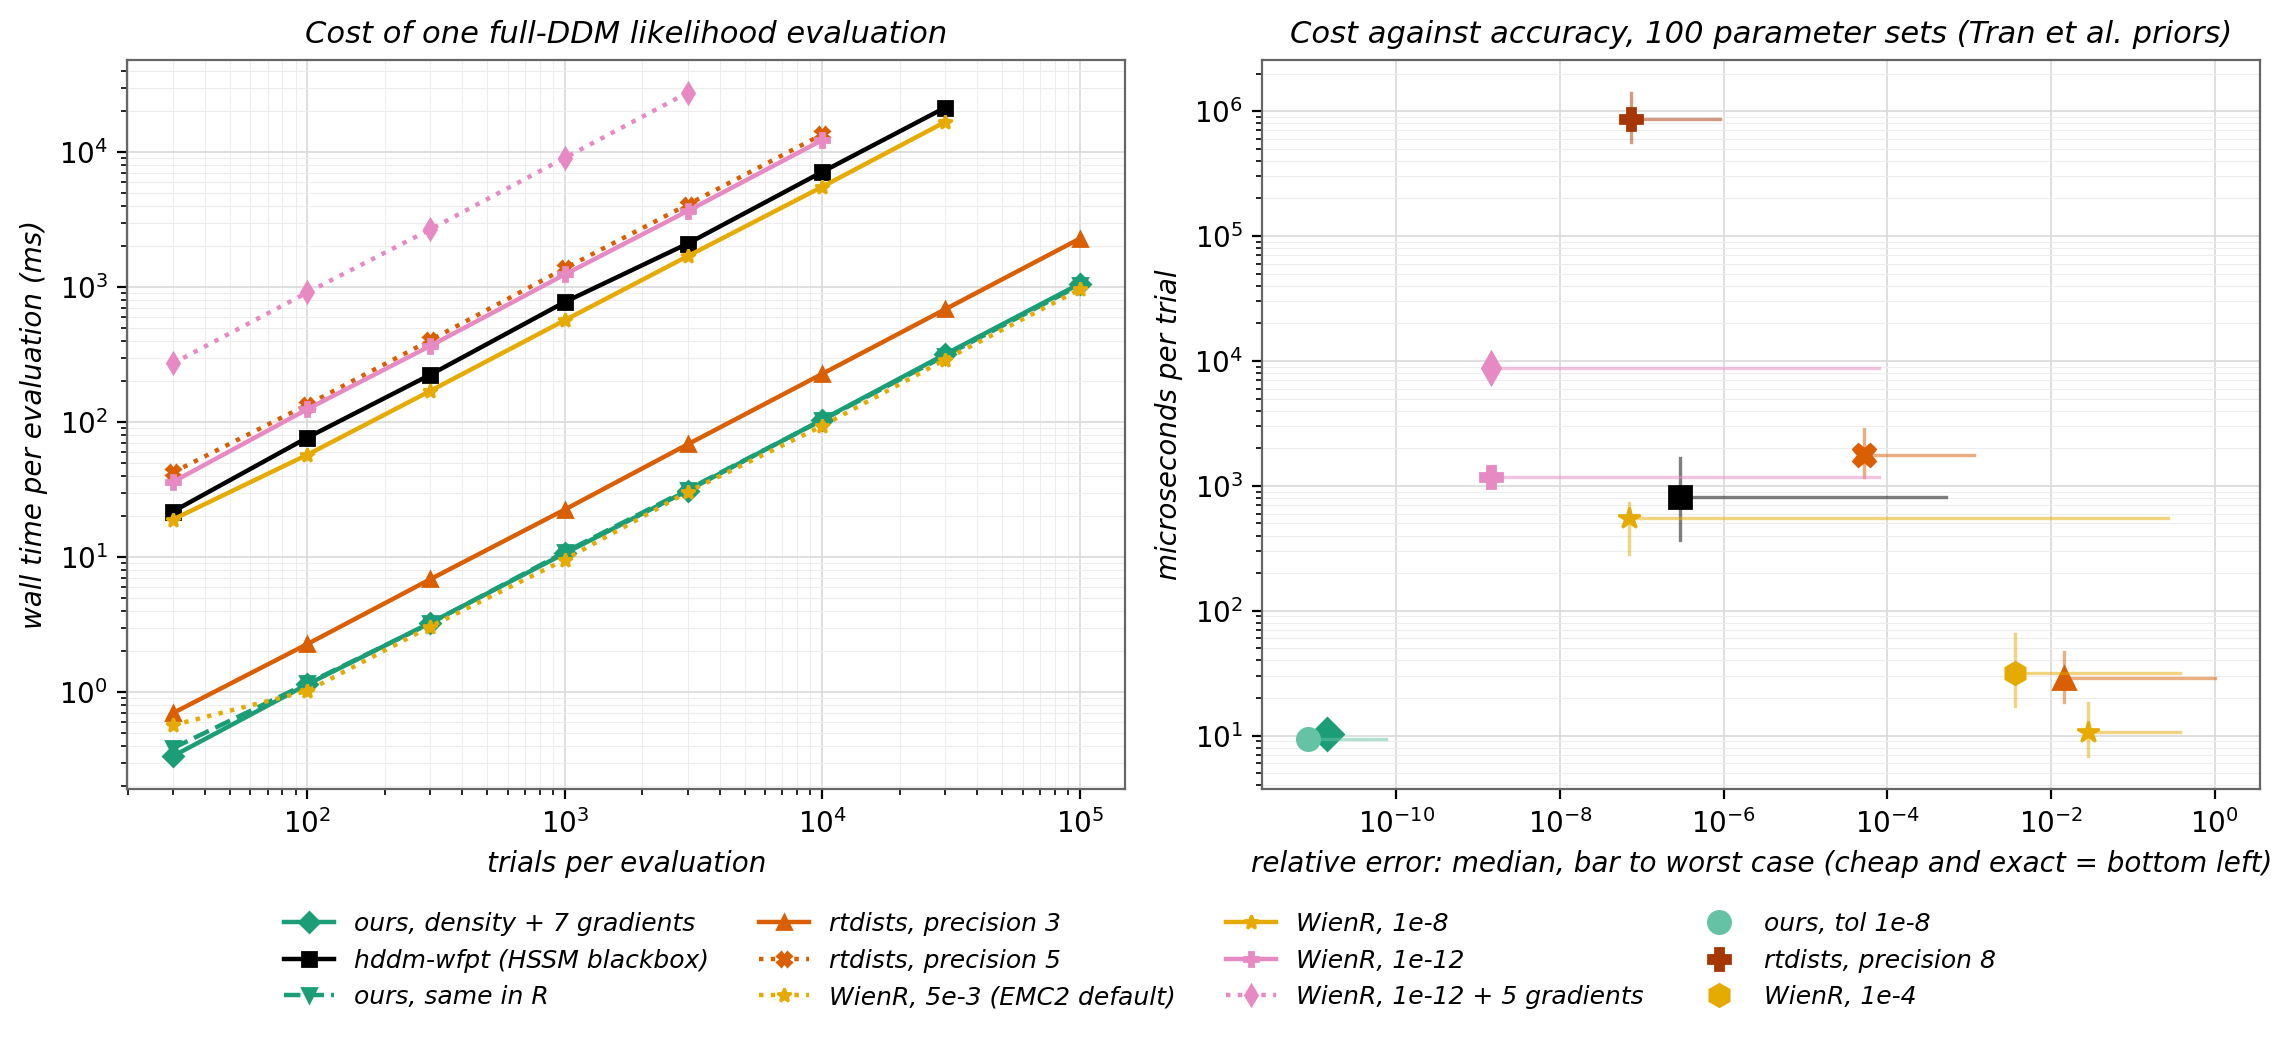
\includegraphics[width=\textwidth]{../fddm-fpt/python/fig_speed_accuracy.png}
\caption{Cost of the seven-parameter likelihood, one thread, on the machine of Table~\ref{tab:timing}. Left: wall time per evaluation against the number of trials, median over five parameter sets. Right: microseconds per trial against relative error on 100 parameter sets drawn from the priors of \citet{tran2021systematic}. Points are medians, horizontal bars run to the largest error, and vertical bars span the middle half of the costs. The error of the closed form is its difference from a 30-digit reference. Each package is run at the settings in the legend.}
\label{fig:frontier}
\end{figure*}

\section{Discussion}

We have shown that the first-passage time density of the diffusion model with normally distributed drift and uniformly distributed starting point has a closed form, and that what makes the integral a Gaussian moment is the factor $\exp(-r_j^2/(2t))$ of the small-time series, which the large-time series lacks. The result completes the analytic treatment of the drift and starting-point integrals of the seven-parameter density. Its distribution function remains a numerical integral, as discussed below.

For the seven-parameter model itself, with the non-decision time uniformly distributed on $[t_0, t_0 + s_t]$, the likelihood is the integral of~\eqref{eq:result} over the non-decision window, Eq.~\eqref{eq:seven} in \ref{app:seven}. We have not found a closed form for that integral, but the reduction is from the two-dimensional numerical integration over starting point and non-decision time used in existing implementations to a one-dimensional quadrature. Because every term of~\eqref{eq:result} and~\eqref{eq:result_large} is a composition of $\exp$, $\Phi$, and $W$, the derivatives of $\gbar$ with respect to $\nu$, $\eta$, $a$, $w_1$, and $w_2$ are in closed form (\ref{app:grad}), where \citet{HartmannKlauer2021} derived them and WienR obtains those involving the variability parameters by one numerical integration per derivative.

For practice the consequences are threefold. The density is exact up to a series truncation error, which has an absolute bound (Section~\ref{sec:conv}) and was checked on 1000 parameter sets (Section~\ref{sec:verify}). It is evaluated at a fixed cost that, in our benchmark, is below that of each of the three packages timed at their own fitting settings. Its partial derivatives are closed form and reuse the exponential factors of the density, which is what gradient-based Bayesian estimation \citep{Wiecki2013, Henrich2024} needs. The across-trial variability parameters are the hardest of the model to estimate \citep{Boehm2018} so a likelihood free of integration over the starting point, with closed-form gradients, removes one source of integration error and gradient noise from that problem, though not its statistical difficulty. The result is directly usable in the packages built on the drift-integrated density~\eqref{eq:geta}, which already contain it as a building block; replacing the quadrature over $w$ by~\eqref{eq:lemma} covers the small-time regime, and a complete implementation also needs the large-time form~\eqref{eq:result_large}, the switch at $t/a^2 = 1$, the stable evaluation of Section~\ref{sec:result}, and the truncation rule~\eqref{eq:JK}. A C++ implementation of~\eqref{eq:result}, \eqref{eq:result_large}, and~\eqref{eq:seven} with all of their derivatives is provided with the paper, with R and Python interfaces that accept the parametrizations of rtdists, WienR, and HSSM, so that it can be called from existing fitting code without conversion.

Unfortunately, the corresponding cumulative distribution function with both forms of variability does not follow by the same route. If one starts from the drift-integrated distribution function of \citet{Blurton2017}, half of the series terms have a coefficient of $w^2$ that is exactly zero after the drift integral and integrate in closed form through $\int\exp(\gamma w)\Phi(\alpha w + \beta)\dd w$; the other half carry the coefficient $+2a^2\eta^2$ (both shown in the supplementary materials), a growing Gaussian times $\Phi$, and reduce to an integral of the form $\int\exp(\kappa' w^2 + \lambda' w)\Phi(\alpha w + \beta)\dd w$ with $\kappa' > 0$, which we have not been able to express in terms of $\exp$ and $\Phi$. For parameter estimation the density suffices. We leave the distribution function open.

\section*{CRediT authorship contribution statement}

\textbf{Kiant\'e Fernandez:} Conceptualization, Methodology, Software, Validation, Formal analysis, Writing -- original draft, Writing -- review \& editing.

\section*{Declaration of competing interest}

The author declares no competing interests.

\section*{Data availability}

All analysis, verification code, and Lean formalization are available in the supplementary material and at \url{https://github.com/kiante-fernandez/ddm-starting-point-closed-form}.

\section*{Funding}

KF is supported by University of California, Los Angeles Dissertation Year Fellowship.

\section*{Declaration of generative AI and AI-assisted technologies in the manuscript preparation process}

During the preparation of this work the author used Claude Fable 5.1 in order to formalize and verify the proofs in Lean. After using this tool, the author reviewed and edited the content as needed and takes full responsibility for the content of the published article.

\appendix

\section{The antiderivative}
\label{app:lemma}

Let $A > 0$, $m = B/A$, and
\begin{align*}
F(w) &:= (p + q m)\sqrt{\frac{2\pi}{A}}\,\exp(C + B^2/(2A))\,\Phi\!\big(\sqrt{A}(w - m)\big) \\
     &\qquad - \frac{q}{A}\,\exp(C + B w - \tfrac12 A w^2).
\end{align*}
Using $\Phi' = \phi$ and $-\tfrac12 A(w - m)^2 + C + B^2/(2A) = C + Bw - \tfrac12 A w^2$,
\begin{align*}
F'(w) &= (p + q m)\sqrt{2\pi}\,\exp(C + B^2/(2A))\,\phi\!\big(\sqrt{A}(w - m)\big) \\
      &\qquad - \frac{q}{A}(B - A w)\,\exp(C + B w - \tfrac12 A w^2) \\
      &= \big[(p + q m) - q(m - w)\big]\,\exp(C + B w - \tfrac12 A w^2) \\
      &= (p + q w)\,\exp(C + B w - \tfrac12 A w^2),
\end{align*}
which is the integrand of~\eqref{eq:lemma}. The definite integral~\eqref{eq:lemma} is $F(w_2) - F(w_1)$. The same computation is carried out symbolically in the supplementary code and formally in the Lean development.

The antiderivative~\eqref{eq:faddeeva} is checked the same way. With $z = \sqrt{\kappa}\,w + \mu/(2\sqrt\kappa)$, so that $2\sqrt{\kappa}\,z = 2\kappa w + \mu$, and $W'(z) = -2zW(z) + 2\I/\sqrt\pi$ \citep[Eq.~7.1.20]{AbramowitzStegun1964},
\begin{align*}
&\frac{\dd}{\dd w}\Big[\exp(\kappa w^2 + \mu w)\,W(z)\Big] \\
 &\quad = \exp(\kappa w^2 + \mu w)\big[(2\kappa w + \mu)W(z) + \sqrt{\kappa}\,W'(z)\big] \\
 &\quad = \exp(\kappa w^2 + \mu w)\,\frac{2\I\sqrt{\kappa}}{\sqrt\pi},
\end{align*}
and multiplying by $-\I\sqrt\pi/(2\sqrt\kappa)$ gives the integrand.

\section{Term bounds}
\label{app:bound}

For $w \in [0, 1]$, $ja \le r_j \le (j+1)a$, and the exponential factor of the prefactor of~\eqref{eq:geta} is bounded by $\exp[(2|\nu|a + \eta^2 a^2)/2S]$. Hence the $j$-th term of the series in~\eqref{eq:geta}, and therefore $|I_j|/(w_2 - w_1)$ in~\eqref{eq:result}, is at most $(j+1)a\exp(-j^2 a^2/(2t))$ times a constant independent of $j$ and $w$. Since $\sum_j (j+1)\exp(-j^2 c)$ converges for every $c > 0$, the series converges absolutely and uniformly in $w$, which justifies the exchange of summation and integration and gives the truncation rule for $J$ in~\eqref{eq:JK}. For $j \ge 2$ and $t \le a^2$ each bound is less than $0.11$ times the one before it, so the sum of all omitted bounds is less than $1.13$ times the first omitted one. The rule~\eqref{eq:JK} makes the exponential factor of that first omitted bound smaller than $\varepsilon$, so the absolute truncation error of~\eqref{eq:result} is below $1.13\,(J+1)\,a\,c\,\varepsilon$. For the large-time series~\eqref{eq:result_large}, $|W(z)| \le 1$ in the closed upper half plane, by the representation $W(z) = \pi^{-1/2}\int_0^\infty \exp(\I z s - s^2/4)\dd s$ for $\operatorname{Im} z \ge 0$, whose integrand has modulus at most $\exp(-s^2/4)$, and $|\exp(\kappa w^2 + \mu_k w)| \le \exp(\kappa + |\lambda|)$ on $[0,1]$, so the $k$-th term is at most a constant times $k\exp(-k^2\pi^2 t/(2a^2))$, which gives the rule for $K$. For $t \ge a^2$ each of these bounds is less than a millionth of the one before it, so the truncation error is essentially the first omitted term.

\section{The seven-parameter likelihood}
\label{app:seven}

With the non-decision time uniformly distributed on $[t_0, t_0 + s_t]$, the density of an observed response time is
\begin{equation}
f(t) = \frac{1}{s_t}\int_{t - t_0 - s_t}^{t - t_0} \gbar\left(u \mid \nu, \eta^2, a, w_1, w_2\right)\dd u ,
\label{eq:seven}
\end{equation}
where the lower limit is replaced by $0$ if negative and $f(t) = 0$ for $t \le t_0$. We have not found a closed form for this integral. In the small-time form the non-decision time shifts the time argument, which enters every term of~\eqref{eq:result} through $\sqrt t$ and $1/t$; in the large-time form it enters through $S$, and only for $\eta = 0$ does the window integrate \citep[Eq.~9]{Tuerlinckx2004}. What~\eqref{eq:result} achieves is to reduce the seven-parameter likelihood from the two-dimensional numerical integration over $(w, u)$ used in existing implementations to a one-dimensional quadrature over $u$ of a smooth closed-form integrand on a short interval. Because $\gbar(u)$ rises steeply from zero at $u = 0$ and the window may include that region, a plain Gauss--Legendre rule converges slowly; the substitution $u = u_{\mathrm{lo}} + (u_{\mathrm{hi}} - u_{\mathrm{lo}})\,\xi^3$, $\xi \in [0, 1]$, with $u_{\mathrm{lo}} = \max(t - t_0 - s_t, 0)$, $u_{\mathrm{hi}} = t - t_0$, and Jacobian $3(u_{\mathrm{hi}} - u_{\mathrm{lo}})\xi^2$, which clusters nodes at the lower limit, fixes this. Table~\ref{tab:nodes} gives the maximum relative error of the rule against adaptive quadrature over the 400 seven-parameter sets of Table~\ref{tab:grid}. A 48-node rule with the cubic map is accurate to ten digits on these sets, at a fixed cost of 48 evaluations of~\eqref{eq:result}. Their smallest $w_1$ is $0.1$. The rule is hardest not where the window is clamped but where $w_1$ is small, since the peak of $\gbar$ sits at a time of order $(aw_1)^2$ and moves inside the window. Table~\ref{tab:w1} gives the error there. Nine digits should be read as holding for $w_1 \ge 0.1$, eight for $w_1 \ge 0.05$, and seven for $w_1 \ge 0.02$. Smaller $w_1$ needs more nodes, which cost only evaluations of a closed form. The gradient of~\eqref{eq:seven} with respect to the five parameters of $\gbar$ is the same rule applied to the closed-form gradient of $\gbar$ (\ref{app:grad}), and $\partial f/\partial t_0 = [\gbar(u_{\mathrm{lo}}) - \gbar(u_{\mathrm{hi}})]/s_t$ and $\partial f/\partial s_t = [\gbar(u_{\mathrm{lo}}) - f]/s_t$ follow from the endpoints when both limits move with the parameters; when the lower limit has been replaced by $0$ it no longer moves, and since $\gbar(0) = 0$ for $w_1 > 0$ the same expressions give the correct values $-\gbar(u_{\mathrm{hi}})/s_t$ and $-f/s_t$. All seven derivatives of~\eqref{eq:seven} agree with central finite differences to ten digits, on a window that lies inside $u > 0$ and on one whose lower limit is replaced by $0$.

\begin{table}[t]
\centering
\caption{Maximum relative error of the 48-node rule with the cubic map for~\eqref{eq:seven}, against adaptive quadrature, at $a = 1.2$, $\nu = \eta = 1$, $w_2 = w_1 + 0.2$, $t_0 = 0.3$, $s_t = 0.25$.}
\label{tab:w1}
\begin{tabular}{lccc}
\toprule
 & \multicolumn{3}{c}{$(t - t_0)/s_t$} \\
\cmidrule(lr){2-4}
$w_1$ & $0.04$ & $0.2$ & $0.8$ \\
\midrule
$0.20$ & $2\times10^{-14}$ & $7\times10^{-15}$ & $2\times10^{-12}$ \\
$0.10$ & $5\times10^{-15}$ & $10^{-12}$ & $2\times10^{-10}$ \\
$0.05$ & $3\times10^{-13}$ & $10^{-10}$ & $4\times10^{-9}$ \\
$0.02$ & $10^{-10}$ & $2\times10^{-9}$  & $10^{-7}$ \\
\bottomrule
\end{tabular}
\end{table}

\begin{table}[t]
\centering
\caption{Maximum relative error of Gauss--Legendre quadrature for~\eqref{eq:seven} against adaptive quadrature, the 400 parameter sets of Table~\ref{tab:grid}, densities above $0.001$.}
\label{tab:nodes}
\begin{tabular}{rcc}
\toprule
Nodes & Plain & With cubic map \\
\midrule
16 & $1.3\times10^{-3}$ & $5.4\times10^{-5}$ \\
24 & $4.2\times10^{-4}$ & $1.5\times10^{-6}$ \\
32 & $7.0\times10^{-5}$ & $8.4\times10^{-8}$ \\
48 & $8.9\times10^{-6}$ & $4.6\times10^{-11}$ \\
\bottomrule
\end{tabular}
\end{table}

\section{Partial derivatives}
\label{app:grad}
Derivatives with respect to the drift variability are taken with respect to $\eta$, as in WienR; the derivative with respect to $\eta^2$ is the same divided by $2\eta$. Differentiating the series term by term is justified by the same Gaussian bounds as the exchange of summation and integration (\ref{app:bound}): since $r_j \le (j+1)a$ and $\partial r_j/\partial a \le j+1$, each derivative of the $j$-th term with respect to $\nu$, $\eta^2$, $a$, or $t$ multiplies the bound of \ref{app:bound} by a polynomial in $j$ of degree at most two, and $\sum_j (j+1)^3\exp(-j^2 c)$ still converges, uniformly on compact parameter sets with $a > 0$ and $t > 0$. The derivatives with respect to the endpoints follow from the fundamental theorem of calculus: $\partial\gbar/\partial w_2 = [g(t \mid \nu, \eta^2, a, w_2) - \gbar]/(w_2 - w_1)$ and $\partial\gbar/\partial w_1 = [\gbar - g(t \mid \nu, \eta^2, a, w_1)]/(w_2 - w_1)$, with $g(t \mid \nu, \eta^2, a, w_i)$ the fixed-start density~\eqref{eq:geta}.

The parameters $\nu$, $\eta$, and $a$ enter $I_j$ only through $A$, $B_j$, $C_j$, $p_j$, and $q_j$. With $E(w) := \exp(-\tfrac12 Aw^2 + Bw + C)$ and the moments $M_n := \int_{w_1}^{w_2} w^n E(w)\dd w$, we have $I = pM_0 + qM_1$, $\partial M_n/\partial B = M_{n+1}$, $\partial M_n/\partial C = M_n$, and $\partial M_n/\partial A = -\tfrac12 M_{n+2}$. Integrating $\frac{\dd}{\dd w}[w^n E(w)]$ over $[w_1, w_2]$ gives
\begin{equation}
A\,M_{n+1} = B\,M_n + n\,M_{n-1} - \big[w^n E(w)\big]_{w_1}^{w_2},
\label{eq:dI}
\end{equation}
so $M_0$, which is~\eqref{eq:lemma} with $p = 1$ and $q = 0$, determines $M_1$, $M_2$, $M_3$, and with them every derivative of $I$. Each parameter derivative is then the chain rule through~\eqref{eq:coef}. For $\nu$ only $B_j$ and $C_j$ depend on the parameter, and
\begin{equation*}
\ddx{\gbar}{\nu} = \frac{1}{(w_2 - w_1)\sqrt{2\pi t^3 S}}\sum_{j=0}^{\infty}(-1)^j \Big[-\frac{a}{S}\,(p_jM_1 + q_jM_2) - \frac{\nu t}{S}\,I_j\Big],
\end{equation*}
with $M_n$ carrying the coefficients of the $j$-th term. Software usually parameterizes the starting point by $w = (w_1+w_2)/2$ and $s_z = a(w_2-w_1)$, for which $\partial\gbar/\partial w = \partial\gbar/\partial w_1 + \partial\gbar/\partial w_2$ and $\partial\gbar/\partial s_z = (\partial\gbar/\partial w_2 - \partial\gbar/\partial w_1)/(2a)$: the first is a sum and is accurate at every width, the second is the difference that the branch of \ref{app:grids} exists to protect. For the large-time representation only two identities are needed, both immediate from $\frac{\dd}{\dd w}\exp(\kappa w^2+\mu w) = (2\kappa w + \mu)\exp(\kappa w^2+\mu w)$: with $\mathcal I := \int_{w_1}^{w_2}\exp(\kappa w^2+\mu w)\dd w$ and $\mathcal E_i := \exp(\kappa w_i^2 + \mu w_i)$,
\begin{align}
\ddx{\mathcal I}{\mu} &= \frac{(\mathcal E_2 - \mathcal E_1) - \mu\,\mathcal I}{2\kappa}, \notag\\
\ddx{\mathcal I}{\kappa} &= \frac{(w_2\mathcal E_2 - w_1\mathcal E_1) - \mathcal I - \mu\,\partial\mathcal I/\partial\mu}{2\kappa}.
\label{eq:dlarge}
\end{align}
Both identities divide by $\kappa = \eta^2 a^2/(2S)$ and lose precision as $\eta \to 0$; at $\eta = 0.001$ they give $\partial\gbar/\partial\eta$ wrong in the third digit. For $\kappa < 0.1$ the implementation in the supplementary material instead expands $\exp(\kappa w^2)$ in powers of $\kappa$, which reduces $\mathcal I$ and its two derivatives to the moments $\int_{w_1}^{w_2} w^n \exp(\mu w)\dd w$. Ten terms give double precision, and the first term is the $\eta = 0$ limit of Section~\ref{sec:large}. All five derivatives agree with the reference of Section~\ref{sec:verify} to fourteen digits for $\eta$ from $0$ to $2$, on both sides of the switch.

\section{Verification grids}
\label{app:grids}

Section~\ref{sec:verify} checks the result on the lattice of Table~\ref{tab:grid}. Two further checks test what that lattice does not reach: the values that published fits of the model actually take, and the limit in which the starting-point range closes to a point.

\emph{Published parameter values.} \citet{tran2021systematic} collected the parameter estimates reported in the diffusion model literature. We draw 2000 parameter sets from those distributions, truncated at the largest and smallest estimate the review records, rejecting any whose starting-point range would cross a barrier, and add 30 fixed points at those extremes. On the scale used here the resulting grid holds boundary separations from $0.11$ to $7.47$, drift rates up to $18.5$ in modulus, drift standard deviations up to $3.45$, mean starting points from $0.04$ to $0.96$, and starting-point ranges from $0.01$ to $0.85$.

We find that on this grid the closed form and WienR agree to ten digits in the density and nine in the five derivatives. The agreement is uniform across the twenty orders of magnitude the density spans, except in the last two rows of Table~\ref{tab:bins}, where it is the reference rather than the series that fails. At five of those 42 sets the two differ in the first digit. Recomputing all five at forty decimal digits shows the closed form correct to twelve digits and WienR not. No evaluation on this grid or on the fixed one, and none in a sweep of 600 response times at every set, returned a negative density.

\emph{A vanishing starting-point range.} Each $I_j$ in~\eqref{eq:result} is a difference of the antiderivative at the two endpoints divided by their separation. As the starting-point range closes, that difference is taken between ever closer values and relative accuracy is lost in proportion. The density degrades slowly, but the derivatives with respect to $w_1$ and $w_2$ are themselves such differences and degrade faster. They are what drives the second column of Table~\ref{tab:width}, which has lost every correct digit at the smallest ranges in the table and is undefined at $w_2 = w_1$. Because $s_z$ is one of the parameters that optimizers and samplers drive towards zero, this is a limit an implementation has to cover.

Existing implementations also treat a vanishing range as a special case. WienR and the Stan implementation skip the integration over the starting point when its range is zero \citep{HartmannKlauer2021, Henrich2024}, and the HDDM likelihood sets any range below $0.001$ to zero and returns the fixed-start density \citep{hddmwfpt}. For those implementations the special case saves time. For~\eqref{eq:result} it is also needed for accuracy. Below a range of $0.01$ we therefore compute $\gbar$ and its gradient as a five-node Gauss--Legendre average of the fixed-start density~\eqref{eq:geta} and its derivatives over $[w_1, w_2]$. The average is a sum rather than a difference, so it loses no digits as the range closes. It holds thirteen digits at every width down to $w_2 = w_1$, where it returns~\eqref{eq:geta} itself. At the threshold it agrees with~\eqref{eq:result} to eleven digits (first row of Table~\ref{tab:width}), whereas setting the range to zero, as HDDM does, would change the density by an amount of the order of the range squared.
\begin{table}[t]
\centering
\caption{Maximum relative difference from WienR on the 2030 parameter sets drawn from the values reported by \citet{tran2021systematic}, by size of the density. One set, at which both give zero in double precision, is omitted.}
\label{tab:bins}
\begin{tabular}{lrc}
\toprule
Density & Sets & Max.\ rel.\ difference \\
\midrule
$10^{-3}$ and above      & 1291 & $8.8\times10^{-12}$ \\
$10^{-6}$ to $10^{-3}$   &  571 & $2.4\times10^{-12}$ \\
$10^{-10}$ to $10^{-6}$  &  125 & $1.6\times10^{-11}$ \\
$10^{-20}$ to $10^{-10}$ &   32 & $2.6\times10^{-1}\,^{\dagger}$ \\
below $10^{-20}$         &   10 & $4.8\times10^{-4}\,^{\dagger}$ \\
\bottomrule
\multicolumn{3}{l}{$^{\dagger}$WienR's integration error, not the closed form's.}
\end{tabular}
\end{table}

\begin{table}[t]
\centering
\caption{Maximum relative difference from a 40-digit reference as the starting-point range closes, over the density and all five derivatives and over four parameter sets including $t = 0.05$ with $a = 2.5$ and $t = 3$ with $a = 0.6$.}
\label{tab:width}
\begin{tabular}{lcc}
\toprule
$w_2 - w_1$ & Eq.~\eqref{eq:result} & Five-node average \\
\midrule
$0.01$     & $5\times10^{-12}$ & $3\times10^{-15}$ \\
$0.001$    & $7\times10^{-10}$ & $3\times10^{-15}$ \\
$10^{-6}$  & $8\times10^{-4}$  & $3\times10^{-15}$ \\
$10^{-8}$  & $4$               & $3\times10^{-15}$ \\
$0$        & undefined         & $10^{-13}$ \\
\bottomrule
\end{tabular}
\end{table}

\section{Supplementary material}

The supplementary material contains (i) an array implementation of~\eqref{eq:result}, \eqref{eq:result_large}, \eqref{eq:seven}, and all partial derivatives in Python, and the C++ implementation of the same with its R and Python interfaces; (ii) the symbolic verification script; (iii) the scripts and reference values for the comparisons with WienR, rtdists, and HDDM, for both grids of \ref{app:grids} and the 1000-set grid of Section~\ref{sec:verify}, and (iv) the Lean formalization.

\bibliographystyle{elsarticle-harv}
\bibliography{refs}

\end{document}
